\section{Графовые алгоритмы – обзор}

\textbf{Графовый алгоритм}  -- алгоритм, предназначенный для обработки и анализа графов и манипуляций с его элементами ???

\textit{Граф} -- это структура данных, представляющая собой множество связанных объектов (вершин), соединенных линиями (ребрами).
\vspace{10pt}

\textit{Алгоритмы поиска/обхода} в графе -- алгоритмы, используемые для систематического обхода или исследования графа. Они помогают найти связи между вершинами, определить кратчайшие пути или выявить определенные свойства графа.

\subsection{Поиск в ширину}
\textbf{Поиск в ширину} \textit{(BFS -- Breadth First Search)} -- фундаментальный алгоритм обхода графа, который исследует вершины графа послойно, начиная от исходной вершины, с целью найти кратчайший путь из одной вершины в другую. В данном случае \textit{кратчайший путь} -- это путь, содержащий наименьшее число ребер.

Алгоритм начинает с истока, посещая все смежные с ним узлы, и только после того, как все соседние узлы посещены, выполняется обход смежных с ними узлов.

\begin{figure}[htbp]
	\centering
	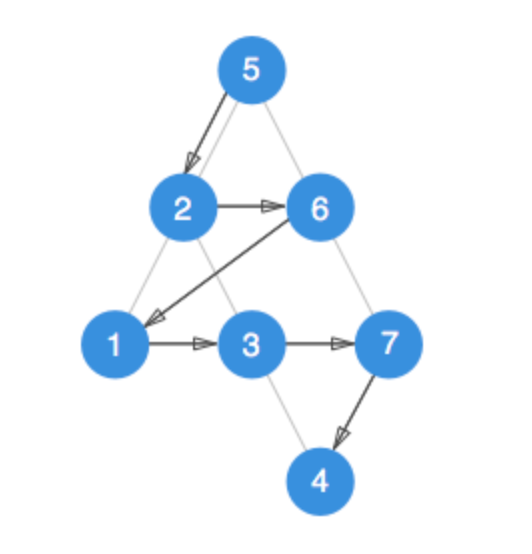
\includegraphics[width=0.4\textwidth]{q35_BFS_representation.png}
	\caption{Графическая визуализация обхода графа в ширину.}
\end{figure}

{\LARGE \textbf{НАПИСАТЬ ПРО ОЧЕРЕДЬ}}
\\[5mm]

Временная асимптотическая сложность алгоритма: 
\begin{itemize}[label=$\triangleright$, font=\scriptsize, noitemsep, topsep=0pt, , partopsep=0pt]
	\item {\footnotesize При использовании списка смежности: \textit{O(n + m)}, где $n$ -- количество вершин в графе, $m$ -- количество ребер.}
	\item {\footnotesize При использовании матрицы смежности: \textit{$O(n^{2})$}, так как алгоритму потребуется полностью перебрать матрицу.}
\end{itemize}
\vspace{5pt}

Пространственная асимптотическая сложность алгоритма: 
\begin{itemize}[label=$\triangleright$, font=\scriptsize, noitemsep, topsep=0pt, partopsep=0pt]
	\item {\footnotesize При использовании списка смежности: \textit{O(n)}, где $n$ -- количество вершин в графе.}
	\item {\footnotesize При использовании матрицы смежности: \textit{$O(n^{2})$}, так как матрица смежности имеет размеры \textit{n * n}.}
\end{itemize}
\vspace{5pt}

{\LARGE \textbf{Добавить код!}}

\subsection{Поиск в глубину}
\textbf{Поиск в глубину} \textit{(DFS -- Depth First Search)} или \textit{эйлеров обход} -- рекурсивный (либо реализованный через LIFO-стек) алгоритм обхода графа, предполагающий исчерпывающий поиск по всем узлам. Алгоритм начинается с заданной вершины графа и проходит по определенному пути так далеко, как только может, и затем возвращается назад, пока не найдет неисследованный путь, чтобы исследовать его. Алгоритм делает это до тех пор, пока не будет исследован весь граф.

\begin{figure}[htbp]
	\centering
	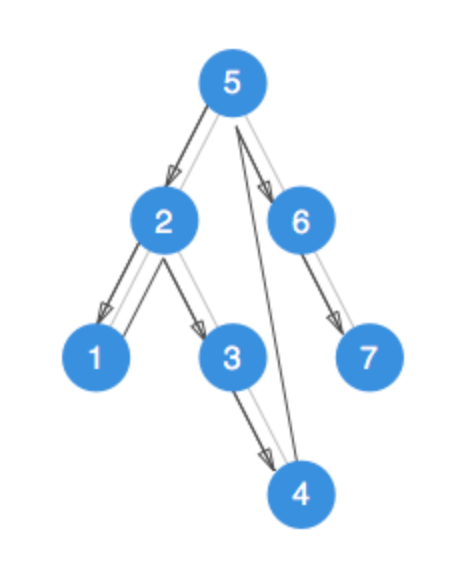
\includegraphics[width=0.4\textwidth]{q35_DFS_representation.png}
	\caption{Графическая визуализация обхода графа в глубину.}
\end{figure}

Асимптотика у поиска в глубину совпадает с ассимптотикой у поиска в ширину.

\subsection{Поиск кратчайшего пути}
\textbf{Поиск кратчайшего пути} в графе -- задача нахождения оптимального пути между двумя вершинами, где путь может быть определен по различным критериям, таким как минимальное количество ребер или минимальный суммарный вес ребер.

Существуют различные алгоритмы для нахождения кратчайшего пути:
\begin{itemize}[label=$\star$, font=\scriptsize, noitemsep, topsep=0pt, partopsep=0pt]
	\item {\footnotesize \textit{Алгоритм Дейкстры}: используется для поиска кратчайших путей во взвешенном графе с \textit{неотрицательными} весами ребер.}
	\item {\footnotesize \textit{Алгоритм Беллмана-Форда}: находит кратчайшие пути во взвешенном графе, в котором есть ребра с \textit{отрицательными} весами.}
	\item {\footnotesize \textit{Алгоритм Флойда-Уоршелла}: используется для нахождения кратчайших путей между всеми парами вершин во взвешенном графе.}
\end{itemize}

{\footnotesize \textit{Примечание.} Необязательно перечислять все три алгоритма в билете, достаточно будет назвать алгоритм Дейкстры и алгоритм Беллмана-Форда.}
\vspace{10pt}

Разберем \textbf{алгоритм Дейкстры}:\\
Алгоритм Дейкстры -- пример  \textit{жадного алгоритма}. На каждом шаге выбирается вершина с минимальным текущим расстоянием от начальной вершины, обновляются расстояния до её соседей и вершина помечается как пройденная. За время работы алгоритма каждый узел графа посещается не более одного раза. Итерации повторяются, пока все вершины не будут посещены или пока не будет найден путь до целевой вершины. \newline

Временная асимптотическая сложность алгоритма Дейкстры: 
\begin{itemize}[label=$\triangleright$, font=\scriptsize, noitemsep, topsep=0pt, partopsep=0pt]
	\item {\footnotesize При использовании двоичной кучи (\textit{binary heap}): \textit{$O(n + mlogn)$}, где $n$ -- количество вершин в графе, $m$ -- количество ребер.}
	\item {\footnotesize При использовании Фибоначчиевой кучи (\textit{Fibonacci heap}): \textit{$O(m + nlogn)$}.}
\end{itemize}
\vspace{5pt}

Пространственная асимптотическая сложность алгоритма Дейкстры: 
\begin{itemize}[label=$\triangleright$, font=\scriptsize, noitemsep, topsep=0pt, , partopsep=0pt]
	\item {\footnotesize При использовании двоичной кучи (\textit{binary heap}): \textit{$O(n + m)$}.}
	\item {\footnotesize При использовании Фибоначчиевой кучи (\textit{Fibonacci heap}): \textit{O(n)}, но есть большая скрытая константа.}
\end{itemize}

\subsection{Нахождение максимального потока}
\textbf{Нахождение максимального потока} по \textit{транспортной сети} -- задача теории графов, в которой требуется определить максимальное количество потока, которое можно пропустить от истока до стока через транспортную сеть с заданными пропускными способностями ребер.

\textit{Транспортная сеть} -- ориентированный граф, в котором каждому ребру присвоена пропускная способность \textit{capacity}.
\vspace{10pt}

Рассмотрим \textbf{алгоритм Диница}:
\begin{enumerate}[font=\footnotesize, noitemsep, topsep=0pt, , partopsep=0pt]
	\item Инициализация потока: для каждого ребра данной сети устанавливается нулевой поток:
	\begin{figure}[htbp]
		\centering
		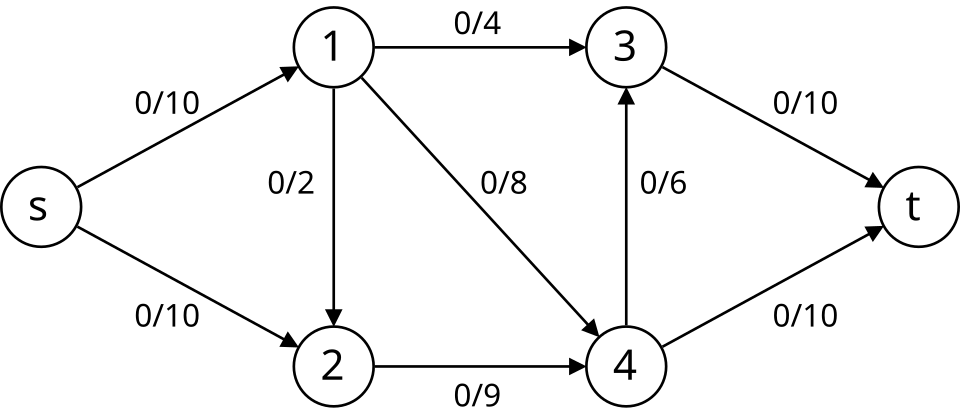
\includegraphics[width=0.4\textwidth]{q35_Dinic_algorithm_representation.png}
		\caption{Графическая визуализация транспортной сети с нулевым потоком.}
	\end{figure}
	\item Построение \textit{слоистой сети} -- разбиение вершин на уровни по расстоянию от истока. При этом ребра, не ведущие на следующий уровень, исключаются.
	\item Поиск \textit{блокирующего потока} -- поток, содержащий насыщенное ребро, то есть этот поток невозможно увеличить. С помощью поиска в глубину анализируем получившуюся в шаге 2 слоистую сеть.
	\item \textit{Обновление потока}. Добавляем найденный блокирующий поток к общему потоку и возвращаемся к шагу 2 до тех пор, пока сток остается достижимым.
\end{enumerate}
\vspace{50pt}



\section{Хеширование, проблемы коллизий}
\textbf{Хеширование} -- процесс преобразования входных данных произвольной длины (ключа) в фиксированный размер выходных данных (хеш-код) с помощью \textit{хеш-функции}.\par
\textit{Хеш-функция} -- функция, преобразующая массив входных данных произвольного размера в выходную строку фиксированной длины, называемую хешем.
\vspace{5pt}

Сферы применения хеширования:
\begin{itemize}[label=$\triangleright$, font=\scriptsize, noitemsep, topsep=0pt, , partopsep=0pt]
	\item {\footnotesize Проверка целостности данных.}
	\item {\footnotesize Поиск в базах данных.}
	\item {\footnotesize Технология блокчейн.}
	\item {\footnotesize Криптография.}
\end{itemize}
\vspace{5pt}

Хеш-функции делятся на две категории: \textit{некриптографические} и \textit{криптографические}.
\begin{itemize}[label=$\triangleright$, font=\scriptsize, noitemsep, topsep=0pt, , partopsep=0pt]
	\item {\footnotesize Некриптографические хеш-функции применяются для оптимизации работы с данными в различных структурах, например, быстрый поиск и хранение информации в хеш-таблицах.}
	\item {\footnotesize Криптографические хеш-функции применяются для защиты данных: кодирование паролей, создание цифровых подписей, аутентификация пользователей.}
\end{itemize}
\vspace{10pt}

Процесс хеширования генерирует хеш фиксированного размера для ключа нефиксированного размера, поэтому существует вероятность, что два ключа могут выдавать одно и то же значение, что приводит к образованию \textit{коллизии}.\par
\textbf{Коллизия} -- событие, при котором хеш-функция генерирует одинаковый хеш-код для двух и более разных входных данных (ключей). Это приводит к тому, что разные данные адресуются в одну и ту же ячейку хеш-таблицы, вызывая конфликт. 
\vspace{5pt}

{\footnotesize \textit{Примечание.}Про методы разрешения коллизий читайте в вопросе \textbf{\ref{sec:collision-handling} \nameref{sec:collision-handling}.}\par
Думаю, на экзамене про методы обработки коллизий также стоит писать и в этом вопросе, чтобы подробнее раскрыть тему коллизий в хешировании.}
\vspace{50pt}



\section{Методы обработки коллизий в хешировании} \label{sec:collision-handling} 

Процесс хеширования генерирует хеш фиксированного размера для ключа нефиксированного размера, поэтому существует вероятность, что два ключа могут выдавать одно и то же значение, что приводит к образованию \textit{коллизии}.\par
\textbf{Коллизия} -- событие, при котором хеш-функция генерирует одинаковый хеш-код для двух и более разных входных данных (ключей). Это приводит к тому, что разные данные адресуются в одну и ту же ячейку хеш-таблицы, вызывая конфликт. 
\vspace{5pt}

Существует два типа методов разрешения коллизий: \textit{метод цепочек} и \textit{открытая адресация}.

\subsection{Метод цепочек} \label{sec:chain_method}

Суть \textit{метода цепочек} закоючается в том, что все элементы, попадающие в одну и ту же ячейку хеш-таблицы, хранятся в виде связанного списка (так называемой \textit{цепочки}).\par
\textbf{Принцип работы:}
\begin{enumerate}[font=\scriptsize, noitemsep, topsep=0pt, , partopsep=0pt]
	\item {\footnotesize \textit{Хеширование ключа}. Ключ обрабатывается хеш-функцией, которая возвращает хеш-код для данного значения.}
	\item {\footnotesize \textit{Обработка коллизий}. Если в ячейке с данным хеш-кодом уже есть элемент, то на этом слоте создается связанный список, в конец которого добавляется новый ключ.}
	\item {\footnotesize \textit{Поиск/удаление элемента}. Вычисляется хеш ключа, находится нужная ячейка, а дальше проводится линейный поиск по цепочке, пока не будет найден элемент с искомым ключом.}
\end{enumerate}
\vspace{5pt}

Временная асимптотическая сложность алгоритма: 
\begin{itemize}[label=$\triangleright$, font=\scriptsize, noitemsep, topsep=0pt, , partopsep=0pt]
	\item {\footnotesize Наихудшая сложность поиска: \textit{O(n)}.}
	\item {\footnotesize Наихудшая сложность удаления: \textit{O(n)}.}
\end{itemize}
\vspace{5pt}

\begin{minipage}[t]{0.45\textwidth}
	\textbf{Преимущества метода:}
	\begin{itemize}[label=$\triangleright$, leftmargin=*, font=\scriptsize, noitemsep, topsep=0pt, , partopsep=0pt]
		\item {\footnotesize Простота реализации.}
		\item {\footnotesize Эффективен при небольшом количестве коллизий.}
		\item {\footnotesize Не требует перестройки таблицы при добавлении элементов.}
	\end{itemize}
\end{minipage}
\hspace{1cm}
\begin{minipage}[t]{0.45\textwidth}
	\textbf{Недостатки метода:}
	\begin{itemize}[label=$\triangleright$, leftmargin=*, font=\scriptsize, noitemsep, topsep=0pt, , partopsep=0pt]
		\item {\footnotesize При большом количестве коллизий списки становятся длинными, из-за чего падает производительность.}
		\item {\footnotesize Затрачивается дополнительная память для хранения указателей на элементы связанных списков.}
	\end{itemize}
\end{minipage}

\subsection{Открытая адресация} \label{sec:open_addressing}

Суть метода \textit{открытой адресации} (или \textit{закрытого хеширования}) заключается в том, что каждый ключ хранится в хеш-таблице исключительно по своему хеш-коду. Каждому хеш-коду соответствует ровно один ключ в хеш-таблице, а размер хеш-таблицы всегда больше количества ключей. Если возникает коллизия, алгоритм ищет следующую свободную ячейку согласно определенной стратегии.
\vspace{5pt}

\begin{minipage}[t]{0.30\textwidth}
	\fontsize{8.5pt}{11pt}\selectfont
	\centerline{\small \textbf{Линейное пробирование}}\par

	Если ячейка занята, то проверяется следующая по порядку:\par
	\vspace{2pt}
	$\boldsymbol{h(k, i) = (h'(k) + i) \ mod \ m}$,\par
	\vspace{2pt}
	где:\par
	\textit{h'(k)} -- исходная кеш-функция,\par
	\textit{i} -- номер попытки,\par
	\textit{m} - размер таблицы.	

	\vspace{6pt}
	\hline
	\vspace{6pt}

	Простая реализация, хорошая локальность кэша, но возникает \textit{кластеризация} -- длинные последовательности занятых ячеек, что ухудшает производительность.
\end{minipage}
\hfill
\begin{minipage}[t]{0.30\textwidth}
	\fontsize{8.5pt}{11pt}\selectfont
	\centerline{\small \textbf{Квадратичное пробирование}}\par

	Если ячейка занята, то проверяется следующая по порядку:\par
	\vspace{2pt}
	$\boldsymbol{h(k, i) = (h'(k) +  c_{1}i + c_{2}i^{2}) \ mod \ m}$,\par
	\vspace{2pt}
	где:\par
	\textit{$c_{1}, c_{2}$} -- константы.

	\vspace{28pt}
	\hline
	\vspace{6pt}

	Уменьшает кластеризацию по сравнению с линейным преобразованием, но может не найти свободную ячейку, даже если она есть (\textit{циклическое пробирование}).
\end{minipage}
\hfill
\begin{minipage}[t]{0.30\textwidth}
	\fontsize{8.5pt}{11pt}\selectfont
	\centerline{\small \textbf{Двойное хеширование}}\par

	Если ячейка занята, то проверяется следующая по порядку:\par
	\vspace{2pt}
	$\boldsymbol{h(k, i) = (h_{1}(k) +  i*h_{2}(k)) \ mod \ m}$,\par
	\vspace{2pt}
	где:\par
	\textit{$h_{2}(k)$} -- вторая хеш-функция, не обращаемая в 0.

	\vspace{17pt}
	\hline
	\vspace{6pt}

	Наиболее равномерное распределение ключей по хешам, минимизированная кластеризация, однако требуется вычисление двух хеш-функций.
\end{minipage}
\vspace{10pt}

\textit{Пару слов об асимптотической сложности:}\par
\begin{itemize}[label=$\triangleright$, font=\scriptsize, noitemsep, topsep=0pt, , partopsep=0pt]
	\item {\footnotesize Средняя сложность поиска: $O(1)$, худший случай: $O(n)$}
	\item {\footnotesize Средняя сложность удаления: $O(1)$, худший случай: $O(n)$}
\end{itemize}
\par
\vspace{5pt}
Асимптотическая сложность алгоритма зависит от \textbf{коэффициента заполнения} таблицы {\mathversion{bold} \(\alpha\)}.
\[
\alpha = \frac{\text{число ключей в таблице}}{\text{размер таблицы}}
\]\par
Оптимальная производительность достигается при $\alpha \leq 0.7$. При таких значениях \alpha \ асимптотика операций остается близкой к $O(1)$.
\vspace{50pt}



\section{Хеш-таблица на основе перемешанной таблицы}
\vspace{-20pt} {\tiny \textbf{\qquad \qquad switch case под капотом!?}}

\textbf{Хеш-таблица} -- это структура данных для хранения пар ключей и их значений. По сути она представляет собой массив, где местоположение элемента массива зависит от значения самого элемента. Связь между значением элемента и его позицией в хеш-таблице задает \textit{хеш-функция}.

\textbf{Перемешанная таблица} -- хеш-таблица, которая использует метод \textit{"\nameref{sec:open_addressing}"} для разрешения коллизий.\par
\vspace{5pt}
{\footnotesize \textit{Примечание}. В билете стоит подробнее расписать метод открытой адресации и основные виды адресации из пункта \ref{sec:open_addressing} \nameref{sec:open_addressing}.}
\vspace{5pt}

\begin{minipage}[t]{0.45\textwidth}
	\textbf{Преимущества перемешанных таблиц:}
	\begin{itemize}[label=$\triangleright$, leftmargin=*, font=\scriptsize, noitemsep, topsep=0pt, , partopsep=0pt]
		\item {\footnotesize Простота структуры данных.}
		\item {\footnotesize Эффективное использование памяти без необходимости создания дополнительных структур данных внутри хеш-таблицы.}
	\end{itemize}
\end{minipage}
\hspace{1cm}
\begin{minipage}[t]{0.45\textwidth}
	\textbf{Недостатки перемешанных таблиц:}
	\begin{itemize}[label=$\triangleright$, leftmargin=*, font=\scriptsize, noitemsep, topsep=0pt, , partopsep=0pt]
		\item {\footnotesize Сложность удаления элементов. Может потребоваться перехеширование оставшихся элементов.}
		\item {\footnotesize Ухудшение производительности при высокой степени заполненности таблицы из-за сложности нахождения свободного хеша для ключа в случае коллизии.}
		\item {\footnotesize Необходимость аккуратного выбора метода пробирования для минимизации кластеризации и улучшения производительности.}
	\end{itemize}
\end{minipage}
\vspace{50pt}



\section{Хеш-таблица на основе связанных списков}
\vspace{-20pt} {\tiny \textbf{\qquad \qquad Как же работает switch case под капотом!?}}

\textbf{Хеш-таблица} -- это структура данных для хранения пар ключей и их значений. По сути она представляет собой массив, где местоположение элемента массива зависит от значения самого элемента. Связь между значением элемента и его позицией в хеш-таблице задает \textit{хеш-функция}.

\textbf{Хеш-таблица на основе связанных списков} строится при помощи \textit{метода цепочек} (подробнее в пункте \ref{sec:chain_method} \nameref{sec:chain_method}), в котором при хешировании в каждую ячейку мы добавляем не ключ, а связанный список ключей.\par
\vspace{5pt}
{\footnotesize \textit{Примечание}. В билете стоит подробнее расписать метод цепочек из пункта \ref{sec:chain_method} \nameref{sec:chain_method}.}
\vspace{5pt}

\begin{minipage}[t]{0.45\textwidth}
	\textbf{Преимущества перемешанных таблиц:}
	\begin{itemize}[label=$\triangleright$, leftmargin=*, font=\scriptsize, noitemsep, topsep=0pt, , partopsep=0pt]
		\item {\footnotesize Не требуется сложная логика пробирования.}
		\item {\footnotesize Гибкость при заполнении таблицы. Производительность не падает при коэффициенте заполнения таблицы $\geq 0.7$.}
		\item {\footnotesize Отсутствие кластеризации.}
		\item {\footnotesize Простота удаления элемента (не требуется перехешировать другие ключи, как при открытой адресации).}
	\end{itemize}
\end{minipage}
\hspace{1cm}
\begin{minipage}[t]{0.45\textwidth}
	\textbf{Недостатки перемешанных таблиц:}
	\begin{itemize}[label=$\triangleright$, leftmargin=*, font=\scriptsize, noitemsep, topsep=0pt, , partopsep=0pt]
		\item {\footnotesize Дополнительные накладные расходны на память из-за необходимости хранения указателей на элементы связанных списков.}
		\item {\footnotesize Сильная зависимость производительности хеш-таблицы от длины связанных списков. Если хеш-функция плохая и все элементы попадают в один бакет, временная сложность деградирует до $O(n)$.}
	\end{itemize}
\end{minipage}
\vspace{50pt}



\section{Построение обратной польской записи выражения}

\textbf{Обратная польская запись} -- это способ записи математических выражений, при котором операторы размещаются после операндов, к которым они применяются. Это отличется от традиционной инфиксной записи, в которой операторы размещаются между операндами.
\vspace{5pt}

\begin{minipage}[t]{0.45\textwidth}
	\centering \textbf{Обратная польская запись:}
	\begin{itemize}[label={}, font=\scriptsize, noitemsep, topsep=0pt, , partopsep=0pt]
	\item \centering \textit{\footnotesize 2 3 * 4 5 * +}
	\item \centering \textit{\footnotesize a b c sin * + d -}
	\item \centering \textit{\footnotesize x 0 > a b ?}
	\end{itemize}
\end{minipage}
\hspace{1cm}
\begin{minipage}[t]{0.45\textwidth}
	\centering \textbf{Инфиксная (обычная) запись:}
	\begin{itemize}[label={}, font=\scriptsize, noitemsep, topsep=0pt, , partopsep=0pt]
	\item \centering \textit{\footnotesize (2 * 3) + (4 * 5)}		
	\item \centering \textit{\footnotesize a + b * sin(c) - d}	
	\item \centering \textit{\footnotesize  (x > 0) ? a : b}
	\end{itemize}
\end{minipage}
\vspace{5pt}

В обратной польской записи нет необходимости в скобках для определения порядка выполнения операций, выражение читается и вычисляется слева направо.
\vspace{5pt}

Преимущества обратной польской записи:
\begin{itemize}[label=$\triangleright$, font=\footnotesize, noitemsep, topsep=0pt, , partopsep=0pt]
	\item {\footnotesize Более простая и эффективная запись для машинной обработки.}
	\item {\footnotesize Не требует использования скобок, что упрощает запись сложных выражений.}
	\item {\footnotesize Позволяет легко реализовывать алгоритмы вычисления выражений с использованием стека.}
\end{itemize}
\vspace{5pt}

\textbf{Алгоритм построения обратной польский записи:}
\begin{enumerate}[font=\footnotesize, noitemsep, topsep=0pt, , partopsep=0pt]
	\item {\footnotesize \textit{Инициализация}. Создаем пустой \textit{стек} для операторов и скобок и \textit{очередь} для выходной ОПЗ.}
	\item {\footnotesize \textit{Посимвольная обработка выражения}:}
	\begin{enumerate}[font=\footnotesize, noitemsep, topsep=0pt, , partopsep=0pt]
		\item {\footnotesize \textit{Элемент -- число или переменная}: добавляем его в выходную очередь.}
		\item {\footnotesize \textit{Элемент -- открывающая скобка \textbf{(}}: помещаем элемент в стек.}
		\item {\footnotesize \textit{Элемент -- закрывающая скобка \textbf{)}}: спускаемся по стеку, перекладывая операторы из стека в выходную очередь, пока не встретим \textbf{(}.}
		\item {\footnotesize \textit{Элемент -- оператор \textbf{+ - / *} и т.д.}: пока в стеке есть операторы с большим или равным приоритетом, перекладываем их в выходную очередь, затем кладем текущий оператор в стек.}
	\end{enumerate}
	\item {\footnotesize \textit{Завершение обработки}. Когда все элементы обработаны, перекладываем все оставшиеся в стеке операторы в выходную очередь.}
\end{enumerate}
Получившаяся выходная очередь -- это и есть \textbf{обратная польская запись}.
\vspace{50pt}



\section{Подходы и инструменты к отладке исходного кода}

\textbf{Отладка исходного кода} -- процесс обнаружения, локализации и исправления ошибок (багов) в коде программного обеспечения, чтобы программа работала так, как от нее ожидается.
\vspace{5pt}

{\centering \textbf{Классификация ошибок в программе:}}\\
\begin{minipage}[t]{0.45\textwidth}
	\begin{center} \textbf{Ошибки времени компиляции (\textit{compilation error}).} \end{center}
	Автоматически выявляются компилятором и не позволяют скомпилировать программу до тех пор, пока ошибки не будут исправлены. Например, \textit{ошибки в синтаксисе}, \textit{неопределенные переменные}, \textit{неверные типы данных} и т.д. Также к ошибкам компиляции относятся ошибки на этапе \textit{линковки}.
\end{minipage}
\hspace{1cm}
\begin{minipage}[t]{0.45\textwidth}
	\begin{center} \textbf{Ошибки времени исполнения (\textit{runtime error}).} \end{center}
	Ошибки, обнаруженные в ходе исполнения программы. К таким ошибкам относятся: \textit{ошибки доступа к памяти}, \textit{ошибки в потоке управления}, \textit{ошибки в логике программы} и др.
\end{minipage}
\vspace{5pt}

\textbf{Основные подходы к отладке:}\par
\begin{enumerate}[font=\footnotesize, noitemsep, topsep=0pt, , partopsep=0pt]
	\item \textit{Логирование} -- запись‍ информации о работе  программы в файлы логов. Позволяет отслеживать процесс разработки, чтобы понять, какие ‌действия выполнялись перед возникновением ошибки.
	\item \textit{Использование отладчиков}. \textit{Отладчики} -- специальные программы, позволяющие выполнять код пошагово, просматривать и изменять значения переменных ​в реальном времени. Примеры отладчиков C++: $GDB$, $LLDB$, $visual \ studio \ debugger$, $clion \ debugger$.
	\item \textit{Профилирование} -- анализ времени выполнения различных частей кода. Помогает выявить узкие места и оптимизировать производительность.
	\item \textit{Unit-тестинг} -- написание‌ и выполнение тестов для отдельных модулей программы. Позволяет оценить корректность работы частей кода и упрощает поиск ошибок.
\end{enumerate}
\vspace{10pt}

{\LARGE \textbf{Еще подумать, что добавить}}.
\vspace{50pt}



\section{Директивы подпрограмм. Неявная рекурсия. Пример}

\textbf{Препроцессор} --- программа для обработки текста перед реальной трансляцией исходного кода в объектный. Может существовать как отдельная программа, так и быть интегрированной в компилятор. В любом случае, входные и выходные данные для препроцессора имеют текстовый формат. Препроцессор преобразует текст в соответствии с директивами препроцессора. Если текст не содержит директив препроцессора, то текст остаётся без изменений.

\textbf{Директивы препроцессора} -- специальные инструкцие для препроцессора, используемые для управления процессом компиляции, условной компиляции, включения файлов и других задач. 
\vspace{5pt}

\textit {Разберем основные виды директивы препроцессора (на примере C/C++)}:
\begin{enumerate}[font=\footnotesize, noitemsep, topsep=0pt, partopsep=0pt]

\vspace{5pt} \hline \vspace{5pt}
	\item \verb|#include| -- включает содержимое другого файла в текущий: \par
	\begin{minted}{cpp}
	#include <stdio.h>  // стандартная библиотека
	#include "svaga.h"  // пользовательский файл
	\end{minted}

\vspace{5pt} \hline \vspace{5pt}
	\item \verb|#define| -- определяет макрос или константу: \par
	\begin{minted}{cpp}
	#define ANSWER_TO_THE_UNIVERSE 42
	#define SVAGA(a, b) ((a) > (b) ? (a) : (b))
	\end{minted}
\textit{Примечание}. Во втором примере директива \verb|#define| используется с аргументами. Такие макроопределения действуют подобно функциям, только никакой вызов функции на самом деле не происходит, а просто на этапе компиляции код макроопределения будет подставлен в код программы.

\vspace{5pt} \hline \vspace{5pt}
	\item \verb|#if|, \verb|#ifdef|, \verb|#ifndef|, \verb|#else|, \verb|#elif|, \verb|#endif| -- директивы условной компиляции: \par
	\begin{minted}{cpp}
	#if VERSION == 1
	    printf("Current version is 1");
	#elif VERSION == 2
	    printf("Current version is 2");
	#else
	    printf("Current version is svaga");
	#endif
	\end{minted}
\textit{Примечание}. Если выражение, стоящее после директивы \verb|#if| оказывается истинным, то будет скомпилирован блок кода, рассположенный между директивами \verb|#if| и \verb|#endif| (или \verb|#elif| и т.п.).

\textbf{\LARGE Еще дописать про неявную рекурсию, директивы #pragma и #error}

\end{enumerate}

